\documentclass{report}
\title{\textsc{\Huge Polar Codes} \\ \textsc{Primary Concepts and
Practical Decoding Algorithms}}

\author{\textbf{Member 1: Himanshu Sharma [1610110149]} \\ \textbf{Member 2: Dhruv Mehra [1610110119]} \\ \textbf{Member 3: Ram Charan [1610110093]} \\\\ {\it Under the guidance of Prof. Vijay K. Chakka} \\\\\\ \LARGE{Dept. of Electrical Engineering} \\\\\\ \textsc{(Endterm Evaluation Report)} \\\\\\\LARGE{Shiv Nadar University} \\ NH91, Tehsil Dadri, Greater Noida, Uttar Pradesh 201314}

\usepackage{float}
\usepackage[margin=1.1in]{geometry}
\usepackage{graphicx}
\usepackage{listings}
\usepackage{color}
\usepackage{amsmath}
 
\definecolor{codegreen}{rgb}{0,0.6,0}
\definecolor{codegray}{rgb}{0.5,0.5,0.5}
\definecolor{codepurple}{rgb}{0.58,0,0.82}
\definecolor{backcolour}{rgb}{0.95,0.95,0.92}

\lstdefinestyle{mystyle}{
    backgroundcolor=\color{backcolour},   
    commentstyle=\color{codegreen},
    keywordstyle=\color{magenta},
    numberstyle=\tiny\color{codegray},
    stringstyle=\color{codepurple},
    basicstyle=\footnotesize,
    breakatwhitespace=false,         
    breaklines=true,                 
    captionpos=b,                    
    keepspaces=true,                 
    numbers=left,                    
    numbersep=5pt,                  
    showspaces=false,                
    showstringspaces=false,
    showtabs=false,                  
    tabsize=2
}

\lstset{frame=tb,
  language=Python,
showstringspaces=false,
  formfeed=newpage,
  tabsize=4,
  morekeywords={models, lambda, forms},
  style=mystyle
}

\begin{document}
\maketitle

\section*{Flowcharts}
\subsection*{Channel Polarization}
Given a B-DMC, the following procedure is followed to polarize the channel.
\begin{figure}[H]
\centering
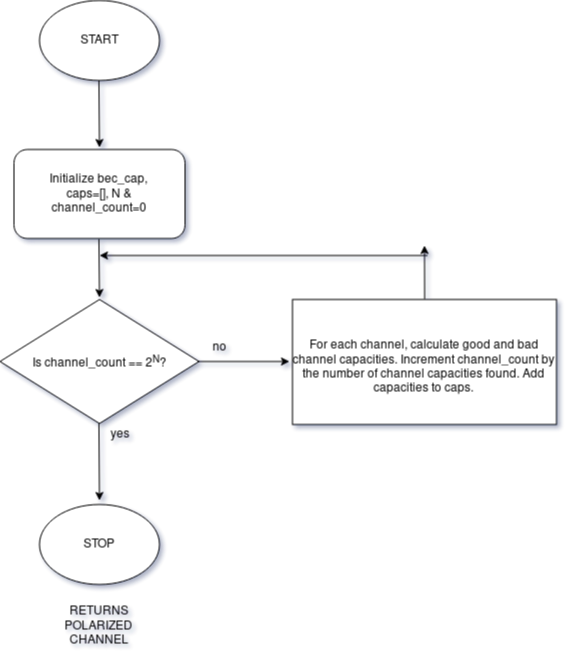
\includegraphics[width=0.6\textwidth, height=0.5\textheight]{code1.png}
\caption{Channel Polarization}
\end{figure}
Basically, once the polarization is done, the channel capacities are generated. A key value pair is generated by the polarize() function. If we want the reliability sequence, then we can use reliability\_sequence() function. Please refer to the first code in the next section.

\section*{Python Codes}
\subsection*{Channel Polarization and Reliability Sequence Generation}
\lstinputlisting[language=Python]{/run/media/chirpcosine/externalhdd/Polar-Codes-in-Digital-Communications/program_codes/channel_polarization.py
}
Let us now take an example run of this code. If we issue the following command 
\begin{lstlisting}
polarize(4) 
\end{lstlisting}
then $2^{4} = 16$ polarized channels will be generated with their respective channel capacities. The output is shown below.
\begin{lstlisting}
{0: 0.9999847412109375, 1: 0.9922027587890625, 2: 0.9853363037109375, 3: 0.7724761962890625, 4: 0.9633636474609375, 5: 0.6538238525390625, 6: 0.5326995849609375, 7: 0.1001129150390625, 8: 0.8998870849609375, 9: 0.4673004150390625, 10: 0.3461761474609375, 11: 0.0366363525390625, 12: 0.2275238037109375, 13: 0.0146636962890625, 14: 0.0077972412109375, 15: 1.52587890625e-05}
\end{lstlisting}
Where, the key indicate the channel number and the values indicate the channel capacity. Let us now generate a reliability sequence for \textbf{5G Standard} with $N=1024$.
\begin{lstlisting}
reliability_sequence(10)
\end{lstlisting}
The output generated is 
\begin{lstlisting}
[577, 545, 529, 521, 517, 515, 514, 513, 385, 321, 293, 291, 290, 289, 281, 277, 275, 274, 273, 269, 267, 266, 265, 263, 262, 261, 260, 259, 258, 257, 201, 197, 195, 194, 193, 177, 169, 165, 163, 162, 161, 153, 149, 147, 146, 145, 141, 139, 138, 137, 135, 134, 133, 132, 131, 130, 129, 113, 105, 101, 99, 98, 97, 89, 85, 83, 82, 81, 77, 76, 75, 74, 73, 72, 71, 70, 69, 68, 67, 66, 65, 57, 54, 53, 52, 51, 50, 49, 47, 46, 45, 44, 43, 42, 41, 40, 39, 38, 37, 36, 35, 34, 33, 31, 30, 29, 28, 27, 26, 25, 24, 23, 22, 21, 20, 19, 18, 17, 16, 15, 14, 13, 12, 11, 10, 9, 8, 7, 6, 5, 4, 3, 2, 1, 297, 209, 55, 516, 78, 58, 518, 84, 79, 59, 519, 86, 522, 87, 322, 61, 523, 90, 323, 100, 91, 136, 305, 525, 102, 325, 140, 530, 103, 93, 142, 531, 106, 148, 143, 107, 225, 150, 533, 329, 151, 109, 154, 641, 114, 164, 155, 115, 166, 546, 537, 167, 157, 547, 117, 170, 264, 171, 337, 549, 268, 386, 270, 387, 173, 121, 196, 276, 271, 178, 198, 278, 389, 179, 553, 199, 279, 202, 282, 181, 292, 203, 283, 578, 393, 294, 579, 32, 295, 205, 285, 48, 353, 210, 298, 185, 581, 56, 561, 211, 299, 80, 60, 769, 520, 88, 62, 524, 213, 324, 301, 92, 63, 306, 401, 526, 585, 326, 104, 94, 307, 532, 527, 327, 144, 108, 95, 226, 534, 330, 152, 217, 110, 227, 309, 642, 535, 331, 156, 116, 111, 538, 643, 168, 158, 548, 118, 229, 539, 333, 593, 172, 159, 338, 550, 119, 645, 313, 388, 174, 417, 339, 122, 551, 272, 541, 390, 180, 175, 554, 123, 200, 280, 233, 391, 182, 341, 555, 204, 284, 649, 394, 580, 183, 125, 296, 206, 286, 354, 395, 186, 582, 557, 609, 562, 212, 300, 207, 287, 770, 355, 187, 345, 583, 563, 214, 302, 241, 64, 397, 771, 402, 586, 449, 308, 215, 528, 328, 303, 357, 657, 96, 189, 403, 587, 565, 218, 228, 310, 536, 773, 332, 112, 644, 219, 230, 311, 405, 540, 334, 594, 589, 160, 120, 361, 646, 314, 418, 340, 231, 552, 569, 335, 542, 595, 176, 777, 221, 124, 234, 647, 315, 673, 419, 392, 342, 556, 543, 409, 650, 184, 126, 235, 597, 396, 343, 558, 610, 369, 317, 208, 288, 651, 421, 356, 188, 127, 346, 584, 564, 242, 785, 398, 772, 559, 237, 611, 450, 216, 304, 358, 658, 347, 190, 601, 404, 705, 588, 653, 566, 243, 399, 774, 451, 425, 359, 659, 613, 220, 191, 312, 406, 590, 567, 349, 362, 775, 801, 245, 232, 570, 336, 596, 453, 778, 222, 407, 648, 591, 661, 316, 674, 420, 363, 433, 617, 544, 410, 571, 236, 598, 779, 223, 249, 344, 675, 370, 318, 457, 652, 422, 833, 128, 411, 365, 665, 786, 599, 573, 560, 238, 612, 625, 781, 371, 319, 423, 677, 348, 602, 706, 654, 244, 400, 413, 787, 465, 452, 426, 239, 360, 660, 614, 897, 192, 603, 373, 568, 707, 655, 350, 681, 776, 802, 246, 427, 789, 454, 615, 481, 408, 592, 662, 605, 351, 709, 364, 434, 377, 618, 803, 247, 572, 429, 689, 455, 793, 780, 224, 250, 663, 676, 458, 435, 619, 713, 834, 805, 412, 366, 666, 600, 574, 251, 626, 782, 459, 372, 437, 320, 621, 424, 835, 678, 367, 667, 721, 809, 575, 414, 788, 466, 253, 627, 240, 783, 461, 441, 679, 898, 837, 669, 604, 374, 737, 817, 708, 656, 415, 467, 682, 629, 428, 790, 899, 841, 375, 616, 482, 469, 683, 633, 606, 352, 710, 378, 791, 901, 804, 248, 849, 430, 483, 690, 456, 473, 794, 685, 607, 711, 379, 664, 905, 865, 436, 431, 691, 485, 620, 714, 795, 806, 381, 913, 693, 252, 489, 715, 797, 807, 460, 438, 622, 836, 929, 368, 668, 722, 697, 497, 810, 717, 576, 439, 623, 254, 628, 961, 784, 723, 811, 462, 442, 680, 838, 670, 255, 738, 818, 725, 813, 463, 416, 468, 443, 839, 630, 671, 739, 819, 729, 900, 842, 445, 631, 376, 741, 821, 470, 684, 843, 634, 792, 745, 825, 902, 471, 850, 845, 635, 484, 753, 474, 903, 686, 608, 851, 637, 712, 380, 906, 475, 687, 866, 853, 432, 692, 486, 796, 907, 477, 867, 857, 382, 487, 914, 909, 869, 694, 490, 383, 716, 798, 915, 808, 873, 695, 491, 799, 930, 917, 881, 698, 498, 493, 718, 931, 921, 699, 440, 499, 624, 719, 962, 933, 724, 701, 812, 501, 963, 937, 505, 256, 965, 945, 726, 814, 464, 969, 444, 840, 727, 815, 672, 977, 740, 820, 730, 993, 446, 731, 632, 447, 742, 822, 733, 844, 743, 823, 746, 826, 472, 846, 636, 747, 827, 847, 754, 749, 829, 904, 852, 638, 755, 639, 757, 476, 688, 854, 761, 855, 908, 478, 868, 858, 488, 479, 859, 910, 870, 861, 911, 384, 871, 916, 874, 696, 492, 875, 800, 918, 882, 877, 919, 494, 883, 932, 922, 495, 885, 700, 923, 500, 720, 889, 934, 925, 702, 935, 502, 703, 964, 938, 503, 939, 506, 966, 946, 941, 507, 967, 947, 509, 970, 949, 728, 816, 971, 953, 978, 973, 979, 994, 981, 732, 995, 985, 997, 448, 734, 1001, 735, 1009, 744, 824, 748, 828, 848, 750, 830, 751, 831, 756, 640, 758, 759, 762, 763, 856, 765, 480, 860, 862, 912, 863, 872, 876, 878, 920, 879, 884, 496, 886, 924, 887, 890, 926, 891, 927, 893, 936, 704, 504, 940, 942, 508, 943, 968, 948, 510, 511, 950, 951, 972, 954, 955, 974, 957, 975, 980, 982, 983, 996, 986, 987, 998, 989, 999, 1002, 1003, 736, 1010, 1005, 1011, 1013, 1017, 752, 832, 760, 764, 766, 767, 864, 880, 888, 892, 928, 894, 895, 944, 512, 952, 956, 958, 959, 976, 984, 988, 990, 991, 1000, 1004, 1006, 1007, 1012, 1014, 1015, 1018, 1019, 1021, 768, 896, 960, 992, 1008, 1016, 1020, 1022, 1023, 1024]
\end{lstlisting}
Why 10 was used? Because $2^{10} = 1024$. The function takes the power as input. Other outputs are discussed in the Channel Polarization section of this report.
\subsection*{Polar Codes Encoding and Decoding}
\lstinputlisting[language=Python]{/run/media/chirpcosine/externalhdd/Polar-Codes-in-Digital-Communications/program_codes/polar_encoding.py}
Using the function monte\_carlo() for $\frac{E_{b}}{N_{o}} = 3 dB$ and $N=16$, $K=8$ with hardcoded reliability sequence $Q$ is shown,
\begin{lstlisting}
monte_carlo(3, 16, 8)
\end{lstlisting}
The output is shown below.
\begin{figure}[H]
\centering
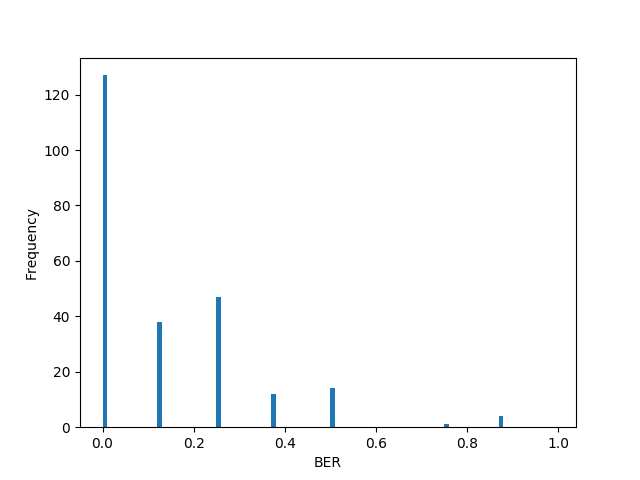
\includegraphics[width=\textwidth, height=0.4\textheight]{hist.png}
\end{figure}
Clearly, most of the times, the BER of polar codes is 0. We now show how the encode() and decode() functions work for polar codes. For  same $N$ and $K$ that we used for the histogram, let us now use encode function.
\begin{lstlisting}
encode(16, 8, Q)
\end{lstlisting}
The output generated is,
\begin{lstlisting}
(array([1, 0, 1, 1, 1, 0, 1, 0]), [1, 0, 0, 0, 0, 1, 1, 1, 1, 1, 0, 1, 0, 0, 1, 0])
\end{lstlisting}
Since $K$ denotes the message bit length, the first element of the array returned is the message stream and the next element is the polar code generated. To decode, take the second element and pass it to decode function.
\begin{lstlisting}
decode([1, 0, 0, 0, 0, 1, 1, 1, 1, 1, 0, 1, 0, 0, 1, 0], Q, 16, 8)
\end{lstlisting}
The output is 
\begin{lstlisting}
[1, 0, 1, 1, 1, 0, 1, 0]
\end{lstlisting}
This is the same message that we sent. \textbf{There are other codes as well. Here we have posted only those codes which are directly related to polar codes.}
\newpage

\section*{Individual Understanding}
\subsection*{By Member 1: Channel Polarization and Reliability Sequence}
Channel polarization is a process in which $N$ channels are generated from $N$ independent copies of a B-DMC $W$. The newly generated channel is $\{W_{N}^{(i)}: 1 \leq i \leq N \}$. As $N \rightarrow \infty$, the symmetric capacity $I(W_{N}^{(i)})$ either becomes 0 or it becomes 1 for all vanishing fractions of $i$. Note that the symmetric capacity of a B-DMC $W$ is given by
\begin{equation}
I(W) = \sum_{x \in X}\sum_{y \in Y}\frac{1}{2}W(y|x)\log_{2}\frac{W(y|x)}{0.5W(y|0) + 0.5W(y|1)}
\end{equation}
\section*{Channel Combining}
Channel combining is a phase operation used in channel polarization wherein \textbf{copies} of B-DMC $W$ are combined in a recursive manner to produce a vector channel $W_{N}: X^{N} \rightarrow Y^{N}$. The value of $N$ is $2^{n}$ where $n \geq 0$. That means, the very first copy of the channel $W_{1}=W$, because $n=0$ for $N=1$. Similarly, $W_{2}: X^{2} \rightarrow Y^{2}$.
\par The transition probability is given by $W_{2}(y_{1}, y_{2}|x_{1}, x_{2})$, note the $W_{2}$, its not $W$. Asking for the value $W_{2}(y_{1}, y_{2}|x_{1}, x_{2})$ is same as asking $W(y_{1}|x_{1})W(y_{2}|x_{2})$, becuase sending $u_{1}$ and $u_{2}$ in channel $W_{2}$ is same as sending $x_{1}$ and $x_{2}$ in two copies of channel $W$ separately. That means,
\begin{center}
$W_{2}(y_{1}, y_{2}|x_{1}, x_{2}) = W(y_{1}|x_{1})W(y_{2}|x_{2}) = W(y_{1}|u_{1}\oplus u_{2})W(y_{2}|u_{2})$ because $x_{1} = u_{1} \oplus u_{2}$.
\end{center}
\begin{figure}[H]
\centering
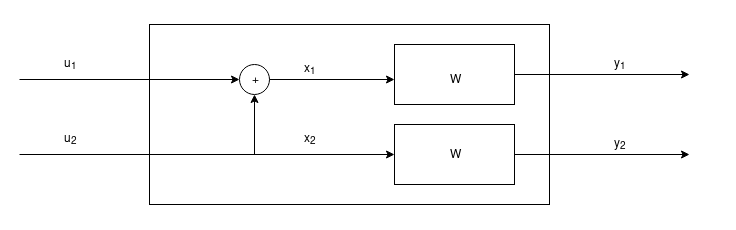
\includegraphics[width=0.8\textwidth, height=0.2\textheight]{twochannel.png}
\caption{Channel $W_{2}$}
\end{figure}
The mapping between $u^{N}$ and $y^{N}$ is done by,
\begin{equation}
y_{i}^{N} = u_{i}^{N}G_{N} \textrm{ }\forall i \in \{1, ...., N\}
\end{equation}
Where
\[G_{2} = 
\begin{bmatrix}
1 & 0 \\
1 & 1
\end{bmatrix}
\]
Similarly, for $W_{4}$ also, the kernel matrix is $G_{4}$ where, 
\[G_{4} = 
\begin{bmatrix}
1 & 0 & 0 & 0 \\
1 & 0 & 1 & 0 \\
1 & 1 & 0 & 0 \\
1 & 1 & 1 & 1
\end{bmatrix}
\]
\begin{figure}[H]
\centering
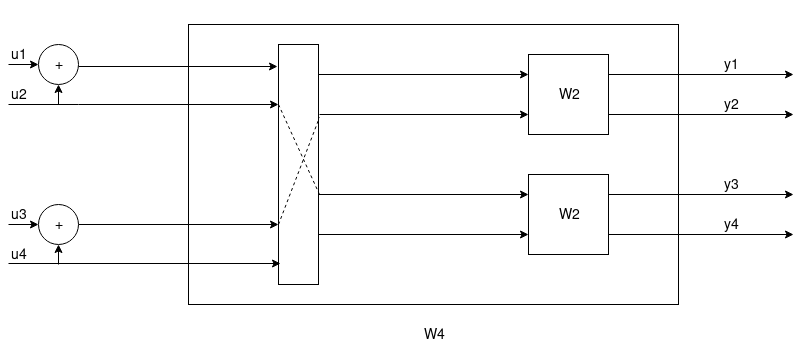
\includegraphics[width=0.8\textwidth, height=0.2\textheight]{w4.png}
\caption{Channel $W_{4}$}
\end{figure}
\begin{figure}[H]
\centering
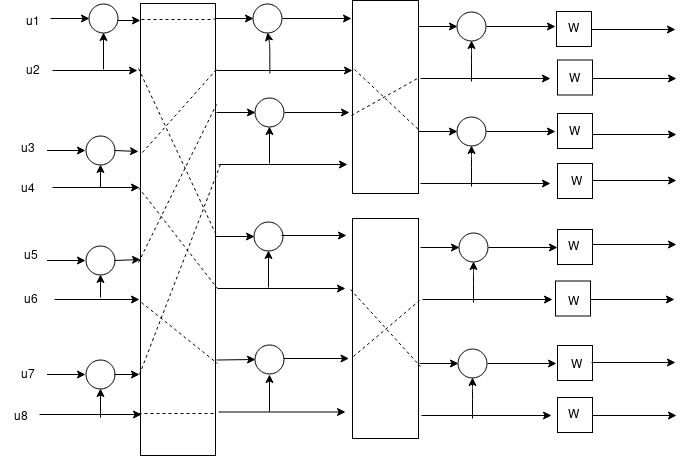
\includegraphics[width=0.8\textwidth, height=0.5\textheight]{w8.png}
\caption{Channel $W_{8}$}
\end{figure}
The vertical rectangular box shown in the channel $W_{4}$ is called the \textbf{reverse shuffle operator} which takes odd indices at one side and even on the other. If one carefully goes through both $W_{4}$ and $W_{2}$, then the outputs $[y_{1}, y_{2},y_{3},y_{4}]$ are $[u_{1}\oplus u_{2} \oplus u_{3} \oplus u_{4}, u_{3} \oplus u_{4}, u_{2} \oplus u_{4}, u_{4}]$. The same can be obtained from the kernel matrix $G_{4}$.
\[
\begin{bmatrix}
u_{1} & u_{2} &u_{3}&u_{4}
\end{bmatrix}
\begin{bmatrix}
1 & 0 & 0 & 0 \\
1 & 0 & 1 & 0 \\
1 & 1 & 0 & 0 \\
1 & 1 & 1 & 1
\end{bmatrix}
=
\begin{bmatrix}
u_{1}\oplus u_{2} \oplus u_{3} \oplus u_{4} & u_{3} \oplus u_{4} &  u_{2} \oplus u_{4} & u_{4}
\end{bmatrix}
\] 

\section*{Channel Polarization}
Channel polarization is a process in which a B-DMC $W$ gives rise to $N$ channels such that $W_{N}^{(i)} \textrm{ } \forall  i \in [1, N]$. In this process, the generated channels either go to zero information state or pure information state of $I(W) = 1/0$ as $N \rightarrow \infty$. The following diagram shows the polarization effect. 
\begin{figure}[H]
\centering
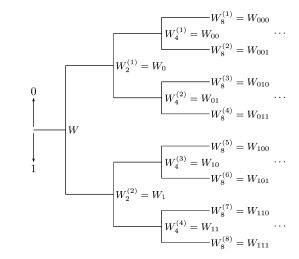
\includegraphics[width=0.4\textwidth, height=0.2\textheight]{chpol.png}
\caption{Channel Polarization Effect}
\end{figure}
Considering the channel $W_{2}$, we can see that it has two copies of the original channel $W$ and therefore, it has a capacity of $2I(W)$ where $I(W) = 1 - f(p)$ is the Shannon's capacity for a BEC and $p$ denotes the transition probability of the BEC.
\subsection*{Single Step Transform}
Consider figure 1 again. This time, refer to the below shown diagram also, taken from the reference. 
\begin{figure}[H]
\centering
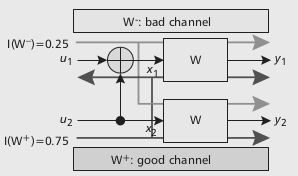
\includegraphics[width=0.4\textwidth, height=0.2\textheight]{w2polar.png}
\caption{Polarized Channel [1]}
\end{figure}
By applying the chain rule of the mutual information, this channel $W_{2}$ can be decomposed into two BEC with capacities $I(W^{-})$ and $I(W^{+})$ where $I(W^{-}) + I(W^{+}) = 2I(W)$. Also, note the following identities,
\begin{equation}
I(W^{-}) = I(W)^{2}
\end{equation}
and 
\begin{equation}
I(W^{+}) = 2I(W) - I(W)^{2}
\end{equation}
In the figure shown above, $I(W)=0.5$. This proves that the bad channel $W^{-}$ has a smaller capacity than the given BEC $W$, whereas the good channel $W^{+}$ has a larger capacity, that is, $I(W^{-} ) \leq I(W) \leq I(W^{+})$. 
\par Let us take over with the same case of $I(W)=0.5$, for BEC $W$. When this channel is polarized once, then $I(W^{-}) = 0.25$ and $I(W^{+}) = 0.75$. Consider `+' to be equivalent of 0 and `-' to be equivalent of 1, then the next will be of order 00, 01, 10, 11, i.e., ++, +-, -+ and --, with following values,
\begin{center}
$I(W^{++}) = 2I(W^{+}) - I(W^{+})^{2} = 0.9375$ \\
$I(W^{+-}) = I(W^{+})^{2} = 0.5625$ \\
$I(W^{-+}) = 2I(W^{-}) - I(W^{-})^{2} = 0.4375$ \\
$I(W^{--}) = I(W^{-})^{2} = 0.0625$ 
\end{center}

As we can see, the more we polarize, the more good and bad channels are generated with their respective channel capacities.
\subsection*{The Matthew Effect}
The Matthew Effect is the summary of channel polarization. It says that as the length of the codeword goes to infinity, the capacity of the most good channel tends to one. The below plot shows the Matthew effect.
\begin{figure}[H]
\centering
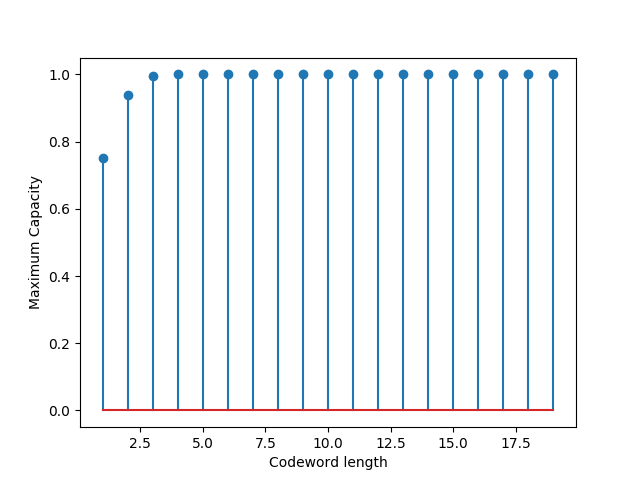
\includegraphics[width=0.8\textwidth, height=0.4\textheight]{matthew.png}
\caption{The Matthew Effect}
\end{figure}
Clearly, as the length of the codeword reaches 3, the capacity of the \textit{good} channel tends to 1. That is, the more codeword length you have, the better will be the capacity of the good channel. Hence, we find that the capacities of most of the polarized channels tend to either 1 (good channels with little noise) or 0 (bad channels with full noise). Equivalently, the error probabilities of the noiseless channels or noisy channels go to 0 or 1. Consider yet another plots for Matthew effect.

\begin{figure}[H]
\centering
\begin{minipage}{0.49\textwidth}
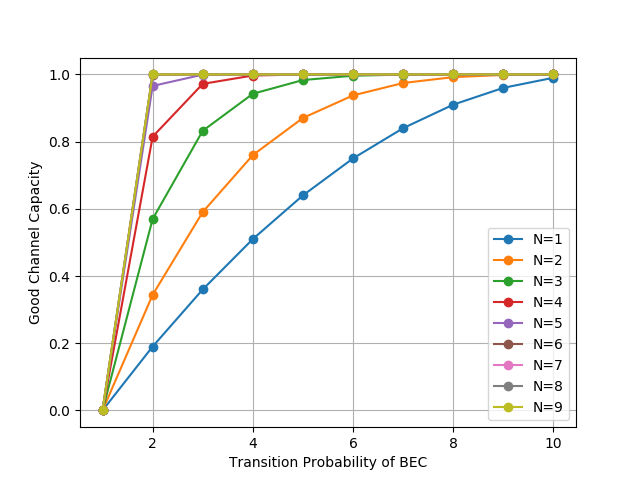
\includegraphics[width=\linewidth]{good_channels.png}
\caption{Good Channels for different levels}
\end{minipage}
\begin{minipage}{0.49\textwidth}
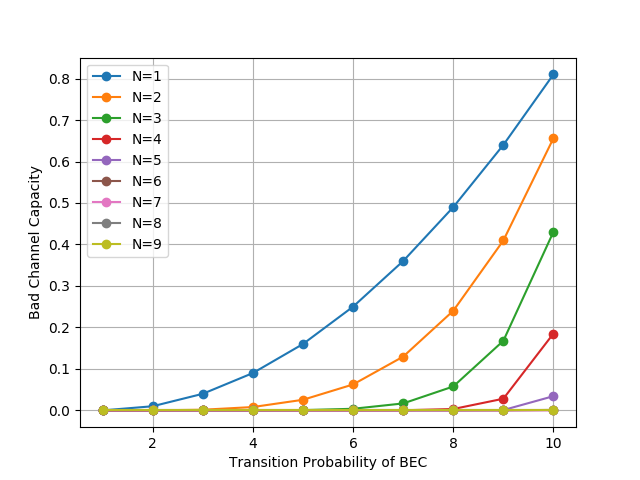
\includegraphics[width=\linewidth]{bad_channels.png}
\caption{Bad Channels for different levels}
\end{minipage}
\end{figure}
Clearly, the larger the $N$ we choose, more quickly the maximum capacity of 1 is achieved. But the case is opposite for bad channels. For bad channels, the lower $N$ you choose, you would be more better off. That is, in a hypothetical case, where we would like to use a noisy bad channel, then according to the figure 8, the best case would be to take the original single copy of the channel at a transitition probability of 0.9. And, for the good channel, we should use as much copies of the original B-DMC at any transition probability from 0.1 to 1.

\section*{Channel Selection and the Reliability Sequence}
Till now, we saw that generating polar codes and polarizing a B-DMC is not a big deal at all. The twist comes when we have to decide what all channels to choose from a given polarized channels. This is given by the reliability sequence. Please refer to the Python codes in this report to know how reliability sequences are generated.

\newpage
\subsection*{By Member 2: Encoding Principles in Polar Codes}
The need for encoding arose due to existence of noisy channels. Since noise reduces the capacity of the channel and increases the error probability, It would be ideal to if we could convert the noisy channel to noiseless. Channel polarization phenomenon suggests a new philosophy for channel coding, i.e selecting the noiseless channels for information-bits transmission.

\subsection*{Linear Block Codes}
An $(n, k)$ binary linear block code is a k-dimensional subspace of the n-dimensional vector space $ V_n =  ( c_0,c_1,...,c_{n-1} ) \, \forall \, C_j \;\; where \;\; C_j \; \epsilon \; GF(2)$.  $n$ is called the length of the code, $k$ the dimension.

\subsection*{Generator Matrix}
\begin{sloppy}
An $(n, k)$ binary linear block codes can be specified by any set of k linear independent codewords $c_0,c_1,. . . ,c_{k-1}$. If we arrange the $k$ codewords into a $k \times n$ matrix $G$, $G$ is called a generator matrix for $C$.\\

Let $u = (u_0,u_1,...,u_{k-1})$, where $u_j \;\epsilon\; GF(2)$$. $$c = (c_0,c_1,. . . ,c_{n-1})= uG$.
The generator matrix $G^{'}$ of a systematic code has the form of $[I_kA]$, where $I_k$ is the $k \times k$ identity matrix. $G^{'}$ can be obtained by permuting the columns of $G$ and by doing some row operations on $G$. We say that the code generated by $G^{'}$ is an equivalent code of the generated by $G$.\\

The basis vectors may be put in a matrix of dimensions $k \times n$, known as the generator matrix, in which every row represents a vector from the coding subspace, and the columns represent corresponding vector components.To encode, the message vector $m = (m_1, m_2,...,m_k)$ has to be multiplied with a generator matrix $G$ to get $c = mG$, where $c(c_1, c_2,...,c_n)$ is a codeword.\\

\subsection*{Hamming Weight and Hamming Distance}
The Hamming weight (or simply called weight) of a codeword $c$, $WH(c)$, is the number of $1$s ( the nonzero components) of the codeword.
The Hamming distance between two codewords $c$ and $c^{'}$ is defined as $dH(c, c^{'})$ $=$ number of components in which $c$ and $c^{'}$ differ.
$dH(c,0)=WH(c)$.\\

Let $HW$ be the set of all distinct Hamming weights that codewords of $C$ may have. Furthermore, let $HD(c)$ be the set of all distinct Hamming distances between c and any codeword. Then, $HW =HD(c)$ for any $c\; \epsilon\; C$. The smallest nonzero element in $HW$ is referred to as $d_{min}$.
$d_{min}$ is the minimum nonzero number of columns in H where a nontrivial linear combination results in zero.

\end{sloppy}

\subsection*{Encoding Principle}
There are mainly three polar encoding schemes: non-systematic, systematic coding, and generalized concatenation coding. The original paper by Arikan mentioned the non systematic version of polar codes. The systematic form was introduced it one of his follow up paper on polar codes. Since the code rate can be finely adjusted by adding or deleting one polarized channel, we can continuously vary the rate of polar codes. Compared with other coding schemes, this rate-compatible property is a significant advantage. Moreover, unlike the traditional code construction to maximize the minimum Hamming distance, the aim of polar coding is to directly minimize the error probability of the information-bearing polarized channels.\\

Polar codes are linear block codes based on the polarization
effect of the kernel matrix \[F_{2} = 
\begin{bmatrix}
1 & 0\\
1 & 1
\end{bmatrix}
\]

A polar code of length $N = 2^n$ and dimension $K$ is defined by the transformation matrix $G_N = F \oplus n$, given by the $n$-fold Kronecker power of the polarization kernel, and a frozen set $F \subset ({1,....,N})$ composed of $N-K$ elements.\\

\subsection*{Non-systematic Scheme}
In The non-systematic codes message bits often do not appear explicitly as such i.e the output does not contain the input symbols.\\

Given the code length $N = 2^n,\; n = 1, 2,....,$ and information length $K$, the binary source block $u = (u_1, u_2, ... , u_N)$ consists of $K$ information bits and $N - K$ frozen bits. The codeword $x$ with code rate $R = K/N$ can be obtained as follows:\\

$x = u$ and $G_N = F \oplus 2$ where $G_N = B_N$ . $F\oplus2$ is the generation matrix, $B_N$ is the bit-reversal permutation matrix, $F2 \oplus2$ is the $n$-th Kronecker power of $F_2$. For non-systematic polar codes, the generator matrix corresponding to the information bits can be composed of the rows of $G_n$ with the lowest error probabilities. In contrast, the Reed-Muller (RM) codes have the similar generation matrix, but the row selection rule is based on the Hamming weight of the rows of $G_N$. the $RM$ rule for information bit assignments leads to asymptotically unreliable codes under SC decoding.\\

Reed-Muller (RM) codes and polar codes are generated by the same matrix $Fn \oplus n$ but using different subset of rows. RM codes select simply rows having largest weights. Polar codes select instead rows having the largest conditional mutual information proceeding top to down in $G_n$; while this is a more elaborate and channel-dependent rule, the top-to-down ordering has the advantage of making the conditional mutual information polarize, giving directly a capacity-achieving code on any binary memoryless symmetric channel (BMSC).\\

For $N = 8$, $K=4$,and $R = 1/2$ The information bits $(u_4, u_6, u_7, u_8)$ are assigned to the polarized channels with the lower error probabilities, while the frozen bits are assigned to the remaining less reliable channels. Each polarized channel is associated with a specific row of the generation matrix. The frozen bits typically take a fixed value of zeros and are assumed known at both the encoder and decoder.\\

The implementation of a decoder utilizes butterfly unit can that can transform two independent input bits $(a, b)$ into two correlated output bits $(a \oplus b, a)$. This operation is recursively applied to the entire codeword, with the codeword getting split into half in each stage until one reaches single source bit $u_i$. So the process of polar coding for $N = 8$ includes one bit reversion and three stages of butterfly operations.

\subsection*{Systemic Scheme}
The generator matrix $G$ of a systematic code has the form of $[Ik A]$, where $I_{k}$ is the $k \times k$ identity matrix.
Polar codes in their standard form are non-systematic codes, in other words, the information bits do not appear as part of the codeword transparently. Since any linear code can be turned into a systematic code, polar codes can also be encoded systematically. Unlike the non-systematic scheme, the information bits appear as part of the codeword transparently in systematic encoding.
However, it is not clear immediately if this can be done while retaining the low-complexity nature of polar coding. It is also unclear at first if there are any significant advantages that arise from systematic encoding of polar codes. With the information bits and the frozen bits at the source block side, the other bits at the codeword side can be determined by some algebraic manipulations. 

We consider coding schemes defined by a linear transformation over a field $F: x=uG$, where $u \in F_{N}$ and $ G \in F_{N \times N}$
In non-systematic coding, u is regarded as the source word and x as the codeword. We can define a family of codes whose rates are adjusted by splitting the source word into two parts $u = (u,u_{c})$ for some $A \subset \{1,...,N\}$ so that the first part $u = (u_{i} : i \in A)$ consists of user data that is free to change in each round of transmission, while the second part $uAc = (u_{i} : i \in Ac)$ consists of digits that are frozen at the beginning of the session and made known to the decoder. The mapping (1) can then be written as
$x=uAGA +uAcGAc$ 
where $GA$ and $GAc$ are the submatrices of G consisting of rows with indices in $A$ and $Ac$, respectively. This mapping defines a non-systematic encoder $uA \rightarrow x = uAGA + c$ where $c =\Delta uAc GAc$ is a fixed vector.
If i fix a code, and consider various possible systematic encoders that code. I can split the codeword into two parts by writing $x = (xB, xBc)$, where $B\subset \{1,...,N\}$, Then:
$xB =uAGAB +uAcGAcB$
$xBc =uAGABc +uAcGAcBc$
where $GAB$ denotes the submatrix of $G$ consisting of the array of elements $(Gi,j)$ with $i \in A$ and $j \in B$, and similarly for the other submatrices. We now seek systematic encoders where $xB$ plays the role $uA$ played in non-systematic encoding as the data carrier, while $uAc$ is fixed as before. More precisely, for any given non-systematic encoder with parameter $(A,uAc)$, we say that a systematic encoder with parameter $(B, uAc)$ exists if equations the above equations can establish a one-to-one correspondence between the sets of possible values of $uA$ and $xB$.
For any polar code defined by some non- systematic encoder with parameter $(A,uAc)$, there exists a systematic encoder with parameter $(B, uAc)$ if (and only if)$A$ and $B$ have the same number of elements and $GAB$ is an invertible matrix.
For any $n \geq 1$, polar codes of block size $N=2^{n}$ can be defined so that they have an encoder with
$G_{N}=F \otimes n$, $F_{n}=[1 1; 0 1]$ 
where $F\otimes n$ denotes the nth Kronecker power of $F$.
It can be observed that $G_{N}$ is lower-triangular with ones on the diagonal, hence it is invertible (in fact, the inverse of $G_{N}$ is itself). For any submatrix $(G_{N})AA$ of $G_{N}$, with $A \subset \{1,...,N\}$, is also lower-triangular and has ones on the diagonal, so it is also invertible.
This implies that the sufficiency conditions hold for polar codes, if we choose $A = B$, to be of non systematic scheme to be into systematic.
\newpage
\section*{By Member 3: Successive Cancellation Decoding}
% Ram Charan's content here

\newpage
\section*{Conclusions}
\end{document}